\documentclass[t]{beamer}
\usetheme{Copenhagen}
\setbeamertemplate{headline}{} % remove toc from headers
\beamertemplatenavigationsymbolsempty

\usepackage{amsmath, array, tikz, bm, pgfplots, tcolorbox, graphicx}
\pgfplotsset{compat = 1.16}
\usepgfplotslibrary{statistics}


\title{Introduction to Probability}
\author{}
\date{}

\AtBeginSection[]
{
  \begin{frame}
    \frametitle{Objectives}
    \tableofcontents[currentsection]
  \end{frame}
}

\begin{document}

\begin{frame} 
\maketitle
\end{frame}

\section{Determine the probability of an event}

\begin{frame}{Sample Space}
\begin{tcolorbox}[colframe=green!20!black, colback = green!30!white,title=\textbf{Sample Space}]
The \textbf{sample space} is a listing of all possible outcomes.
\end{tcolorbox}
\vspace{6pt} \pause
\onslide<+->{Common sample spaces:} \\
\begin{itemize}
	\item<+->{\emph{Flipping a coin}: Heads, Tails}
	\item<+->{\emph{Rolling a single die}: 1, 2, 3, 4, 5, 6}
	\item<+->{\emph{Drawing a card from a standard deck}: Ace of spades, ace of hearts, $\dots$, king of diamonds}
\end{itemize}
\end{frame}

\begin{frame}{Venn Diagrams}
\begin{tcolorbox}[colframe=green!20!black, colback = green!30!white,title=\textbf{Venn Diagrams}]
A \textbf{Venn diagram} is a visualization of events and sample spaces.
\end{tcolorbox}
\vspace{8pt} \pause
\begin{center}
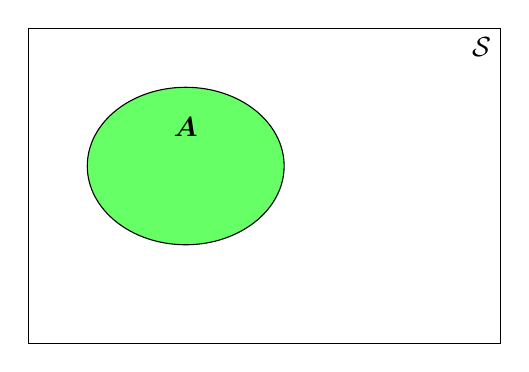
\begin{tikzpicture}
\draw (0,0) rectangle (6,4);
\draw [fill=green!60] (2,2.25) ellipse (1.25cm and 1cm);
\node at (6,4) [below left] {$\mathcal{S}$};
\node at (2,2.75) {$\bm{A}$};
\end{tikzpicture}
\end{center}
\end{frame}

\begin{frame}{Playing Cards}
\begin{center}
\includegraphics[scale=0.23]{../Images/Playing_Cards.png}
\end{center}
\end{frame}

\begin{frame}{Probability}
\begin{tcolorbox}[colframe=green!20!black, colback = green!30!white,title=\textbf{Probability}]
\textbf{Probability} is a measure of the likelihood of an event occurring.
\end{tcolorbox}
\vspace{6pt} \pause
\begin{center}
Probability = $\dfrac{\text{number of ways the event can occur}}{\text{total number of outcomes in sample space}}$
\end{center}
\end{frame}

\begin{frame}{Example 1}
Determine the probability of each event.	\newline\\
(a)	\quad	Flipping a coin and landing on heads \newline\\	\pause
1 outcome: Heads	\quad \pause 2 outcomes in sample space \pause
\[P(\text{heads}) = \frac{1}{2}\]
\end{frame}

\begin{frame}{Example 1}
(b)	\quad Rolling a number less than 3 on a single die.	\newline\\	\pause
2 outcomes: 1, 2	\quad	\pause	6 outcomes in sample space \pause
\[P(\text{rolling less than 3 on a single die}) = \frac{2}{6} = \frac{1}{3} \]
\end{frame}

\begin{frame}{Example 1}
(c)	\quad	Drawing a face card from a standard deck.	\newline\\	\pause
Face cards include jacks, queens, and kings. \newline\\	\pause
There are four suits for each card: clubs, diamonds, hearts, and spades.	\newline\\	\pause
Thus, there are 12 total face cards: jack of clubs, jack of diamonds, $\dots$, king of spades	\quad \pause There are 52 total cards	\pause
\begin{align*}
P(\text{drawing a face card}) &= \frac{12}{52} \\[6pt]	
P(\text{drawing a face card}) &= \frac{3}{13}
\end{align*}
\end{frame}

\begin{frame}{Example 1}
(d)	\quad The number of students in each class at a college is shown in the table below.
\begin{center}
\begin{tabular}{cccc}
Freshmen	&	Sophomore	&	Junior	&	Senior	\\	\hline
1670		&	2017		&	2975	&	3026	
\end{tabular}
\end{center}
Find the probability that a randomly selected student is a sophomore.	\newline\\	\pause

Out of the 9,688 students attending the college, 2,017 of them are sophomores.	\newline\\	\pause

\[P(\text{sophomore}) = \frac{2017}{9688} \]
\end{frame}

\begin{frame}{Example 1}
(e)	\quad The 36 possible sums from rolling 2 dice are shown below.
\begin{center}
\begin{tabular}{c|cccccc}
			&	\textbf{1}	&	\textbf{2}	&	\textbf{3}	&	\textbf{4}	&	\textbf{5}	&	\textbf{6}	\\ \hline
\textbf{1}	&		2		&		3		&		4		&		5		&		6		&		7		\\
\textbf{2}	&		3		&		4		&		5		&		6		&		7		&		8		\\
\textbf{3}	&		4		&		5		&		6		&		7		&		8		&		9		\\
\textbf{4}	&		5		&		6		&		7		&		8		&		9		&		10		\\
\textbf{5}	&		6		&		7		&		8		&		9		&		10		&		11		\\
\textbf{6}	&		7		&		8		&		9		&		10		&		11		&		12
\end{tabular}
\end{center}

What is the probability of rolling a sum of 7?
\begin{align*}
\onslide<2->{P(\text{sum of 7}) &= \frac{6}{36}} \\[8pt]
\onslide<3->{&= \frac{1}{6}}
\end{align*}
\end{frame}

\section{Find the experimental probability of an event}

\begin{frame}{Types of Probability}
In the previous examples, each outcome had an equal chance of being selected. This is referred to as {\color{red}\textbf{classical probability}}.	\newline\\	\pause

There are two other types of probability: experimental and subjective.
\end{frame}

\begin{frame}{Experimental and Subjective Probabilities}
\begin{tcolorbox}[colframe=green!20!black, colback = green!30!white,title=\textbf{Experimental Probability}]
\textbf{Experimental probability} is probability based on events that have actually occurred.
\end{tcolorbox}
\vspace{10pt}	\pause
\begin{tcolorbox}[colframe=green!20!black, colback = green!30!white,title=\textbf{Subjective Probability}]
\textbf{Subjective probability} is probability based on opinion.
\end{tcolorbox}
\end{frame}

\begin{frame}{Example 2}
Flip a coin 10 times and state the experimental probability of landing on tails.
\end{frame}

\begin{frame}{Law of Large Numbers}
As the number of events increases, the experimental probability of an event will approach the classical (a.k.a. \textit{theoretical}) probability.
\end{frame}

\begin{frame}{Rules of Probability}
Rules of Probability Club:	\newline\\ \pause
\begin{itemize}
	\item<+-> Each probability must be a value between 0 and 1, inclusive.
	\begin{itemize}
		\item<+-> A probability of 0 is an \textit{impossible event}.
		\item<+-> A probability of 1 is a \textit{certain event}.
	\end{itemize}
	\item<+-> The sum of all possible probabilities of a sample space must equal 1.
\end{itemize}
\end{frame}



\end{document}